% \documentclass[journal]{vgtc}                % final (journal style)
% \documentclass[review,journal]{vgtc}         % review (journal style)
% \documentclass[widereview]{vgtc}             % wide-spaced review
% \documentclass[preprint,journal]{vgtc}       % preprint (journal style)
% First we choose the document class (can be book, report, article etc.)
\documentclass[11pt]{article}
% \documentclass[11pt, twocolumn]{elsarticle}
% \documentclass{ieeetran}

\usepackage{mathtools} % Math
\usepackage{amssymb} % More Math symbols
\usepackage{textgreek} % Greek letters inline with text
\usepackage{graphics} % Images
\usepackage{pythonhighlight} % Syntax Highlighted code
\usepackage[margin=0.6in]{geometry} % Change Margins
\usepackage[shortlabels]{enumitem} % Enum with letters

% \ifpdf%                                % if we use pdflatex
%   \pdfoutput=1\relax                   % create PDFs from pdfLaTeX
%   \pdfcompresslevel=9                  % PDF Compression
%   \pdfoptionpdfminorversion=7          % create PDF 1.7
%   \ExecuteOptions{pdftex}
%   \usepackage{graphicx}                % allow us to embed graphics files
%   \DeclareGraphicsExtensions{.pdf,.png,.jpg,.jpeg} % for pdflatex we expect .pdf, .png, or .jpg files
% \else%                                 % else we use pure latex
%   \ExecuteOptions{dvips}
%   \usepackage{graphicx}                % allow us to embed graphics files
%   \DeclareGraphicsExtensions{.eps}     % for pure latex we expect eps files
% \fi%

%% it is recomended to use ``\autoref{sec:bla}'' instead of ``Fig.~\ref{sec:bla}''
% \graphicspath{{figures/}{pictures/}{images/}{./}} % where to search for the images
\usepackage{microtype}                 % use micro-typography (slightly more compact, better to read)
\PassOptionsToPackage{warn}{textcomp}  % to address font issues with \textrightarrow
\usepackage{textcomp}                  % use better special symbols
\usepackage{mathptmx}                  % use matching math font
\usepackage{times}                     % we use Times as the main font
\renewcommand*\ttdefault{txtt}         % a nicer typewriter font
\usepackage{cite}                      % needed to automatically sort the references


\title{Title of my document}
% \date{2019-0}
\author{Flavio R. de A. F. Mello}


%% Paper title.
% \title{Global Illumination for Fun and Profit}

%% This is how authors are specified in the journal style

%% indicate IEEE Member or Student Member in form indicated below
% \author{Roy G. Biv, Ed Grimley, \textit{Member, IEEE}, and Martha Stewart}
% \authorfooter{
% %% insert punctuation at end of each item
% \item
%  Roy G. Biv is with Starbucks Research. E-mail: roy.g.biv@aol.com.
% \item
%  Ed Grimley is with Grimley Widgets, Inc.. E-mail: ed.grimley@aol.com.
% \item
%  Martha Stewart is with Martha Stewart Enterprises at Microsoft
%  Research. E-mail: martha.stewart@marthastewart.com.
% }

%other entries to be set up for journal
% \shortauthortitle{Biv \MakeLowercase{\textit{et al.}}: Global Illumination for Fun and Profit}

% \abstract{Duis au}

% Now we start the main document stuff
\begin{document}

\maketitle

\section{Domain and Task}
    This work aims to study the implementation of a Reinforcement Learning algorithm in a multi-agent scenario. For this study, a simple task was devised: agents are randomly placed in the playing field and their goal is to reach a particular desired arrangement. The environment is discrete, static, and fully observable by all agents. States are deterministic and episodic in nature.

\subsection{Playing Field Arrangement}
    The field consists of 7 locations arranged in a cross-shaped form.

    \begin{figure}[h]
        \centering
        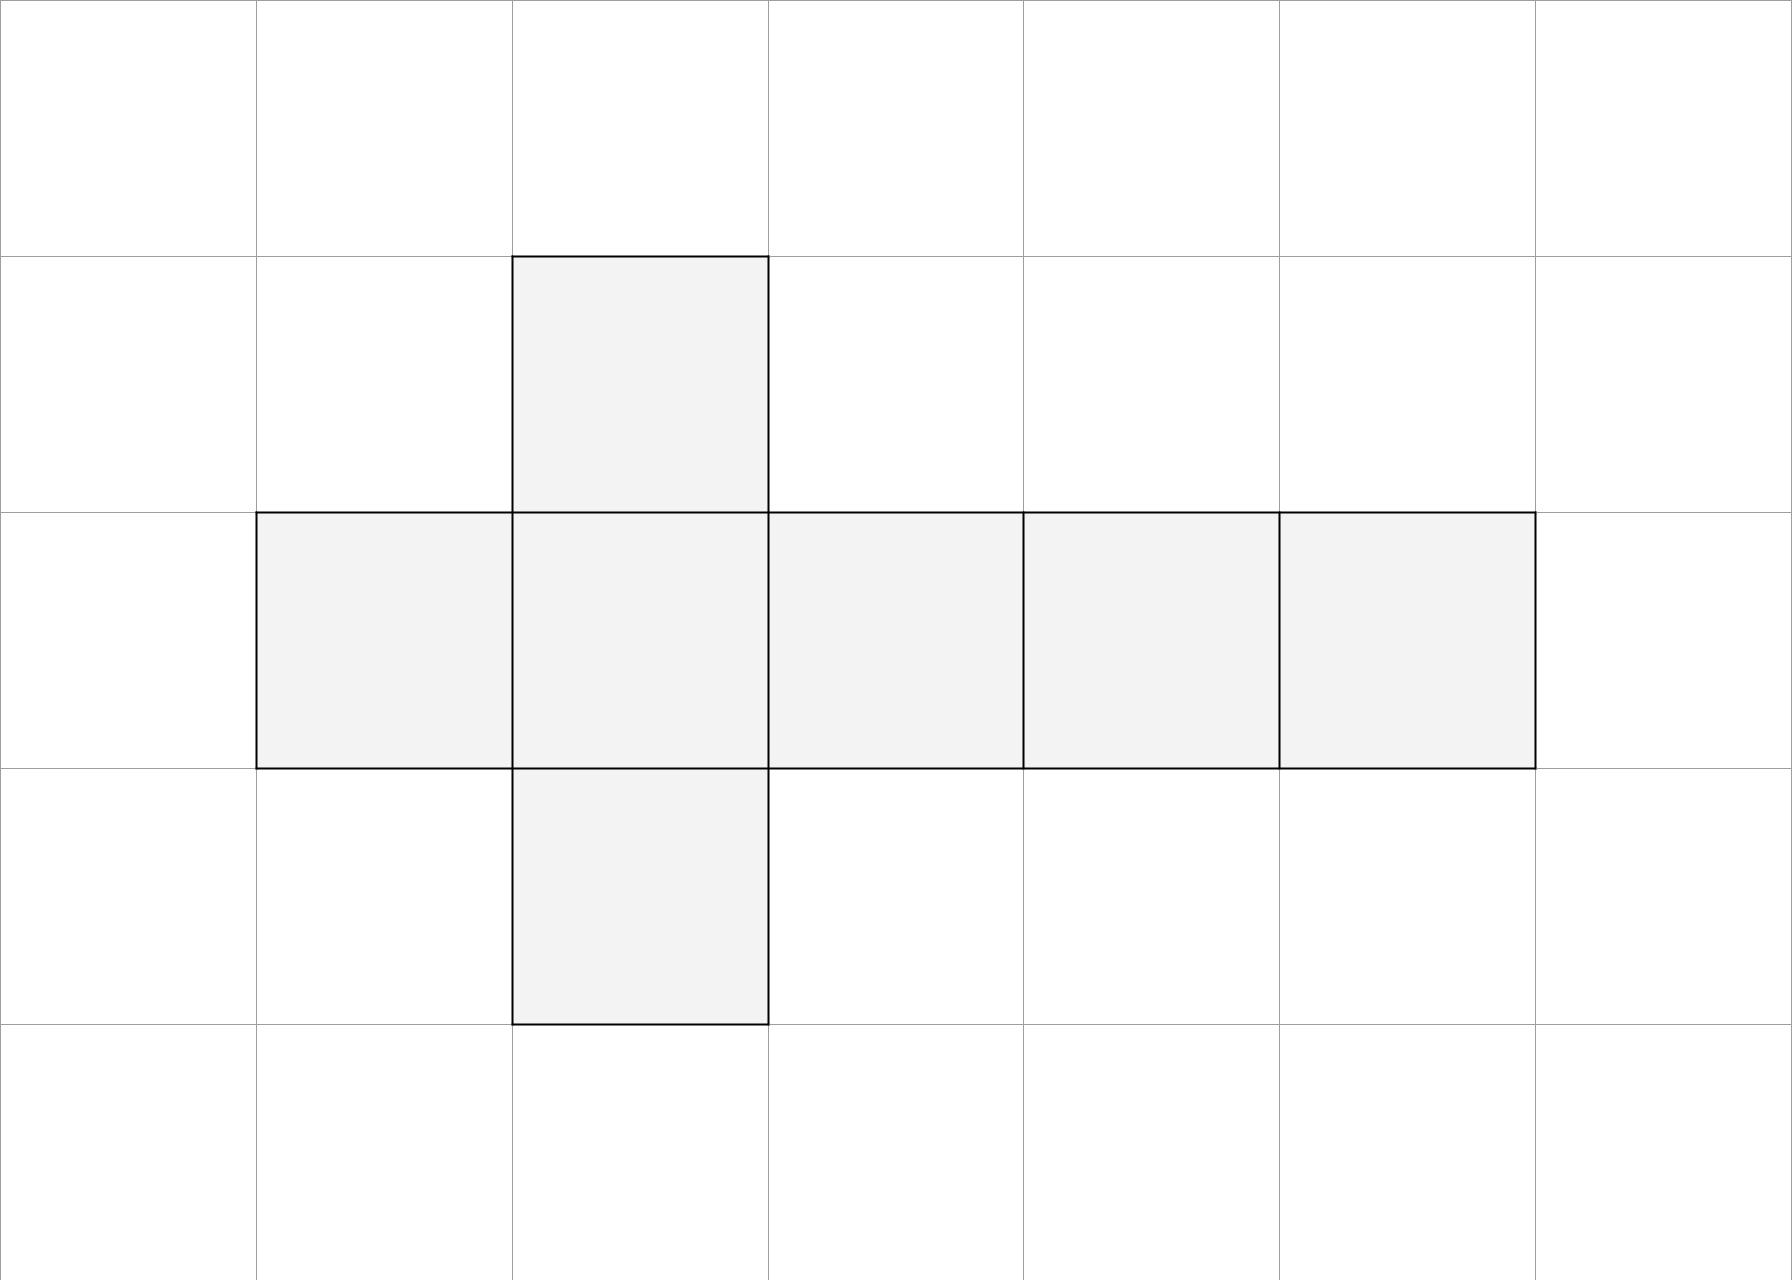
\includegraphics[height=4cm]{./Images/1_Playing_Field.jpg}
        \caption{Visual representation of the playing field}
    \end{figure}

\subsection{Playing Rules}
    Each action consists of a move to an adjacent location. Moves are only allowed in the cardinal directions, no diagonal moves are allowed. Multiple agents may not occupy a same location at the same time, therefore moves are only allowed if the destination is an empty location. Alternatively, agents may elect to stay in the same place. Thus, there are 5 possible actions: move up, move right, move down, move left, and stay in the same place. It is important to note that the field topology plays a role in determining which actions are possible for a given agent in a given state. It is perfectly possible for agents' action options be reduced to staying in place for a specific state. Agents will take turns performing actions, starting with agent 1.

\subsection{Task Goal}
    The goal is to have the agents reach the rightmost section of the field in ordered section. The agent with the smallest id number is to be at the rightmost square, followed by the other agents successively. The rightmost section is a narrow corridor, this setup allows for situations where a given agent may block the passage of the other. This characteristic of the playing field was intentionally designed to require for cooperation between agents. If they directly move to their final position, one agent may be blocking the another agent's path and thus fail to reach the final desired state.

% // IMAGE task goal for 1, 2 & 3 agents


\section{State Transition and Reward Functions} \label{sec:transition}
    For implementation purposes, the states are encoded into a single string of 7 characters. Agents are assigned ids in the form of positive numbers, which are used to indicate their position in the field. the value `0` is reserved for empty spaces. Each of the 7 locations is assigned an id from 0 through 6, which is used to map the location with the index in the encoded string. Figures \ref{fig:field_indexed} and \ref{fig:field_mapping} show the location indexes and an example of the mapping between a state string and its equivalent board arrangement.


    \begin{figure}[h]
        \centering
        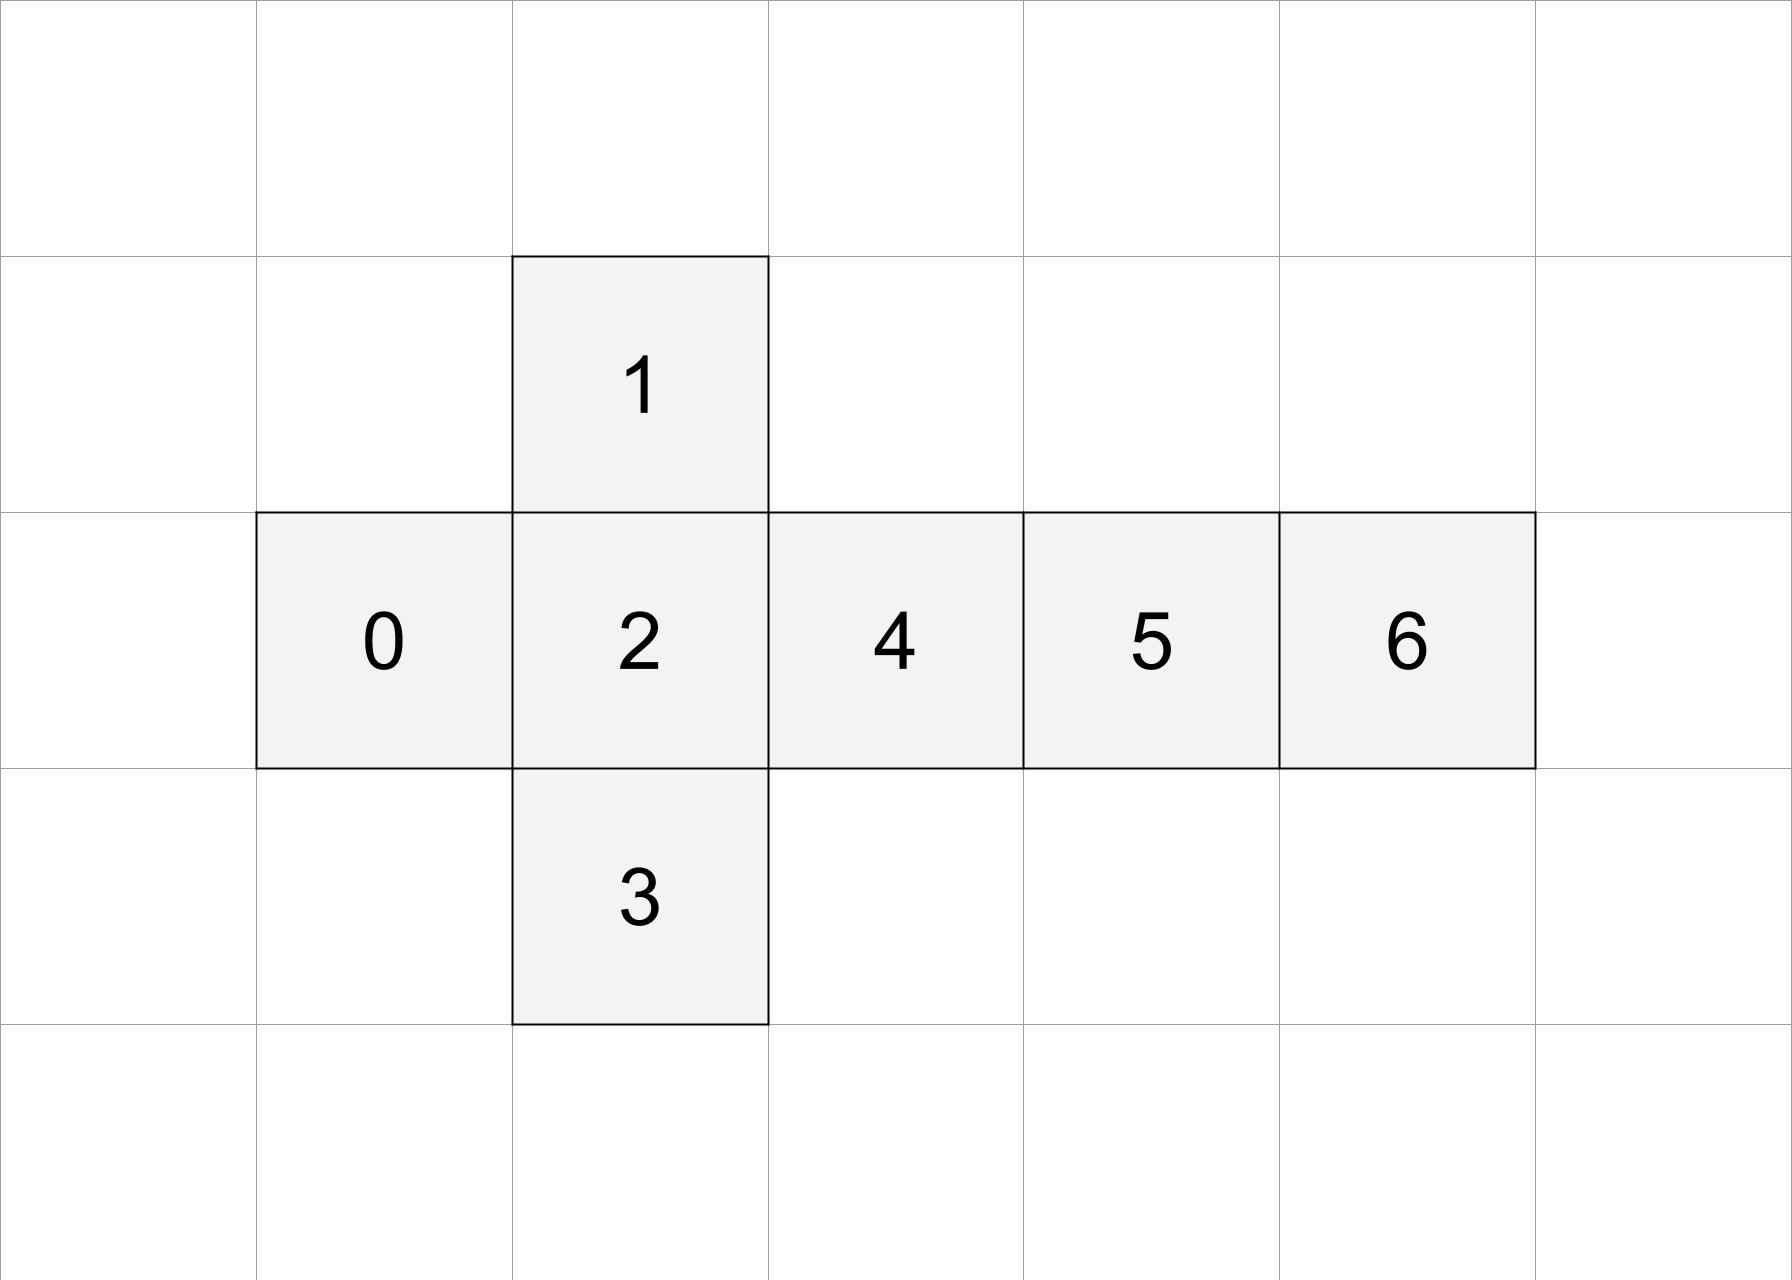
\includegraphics[height=4cm]{./Images/2_Playing_Field_Indexed.jpg}
        \caption{Playing field with location ids}
        \label{fig:field_indexed}

        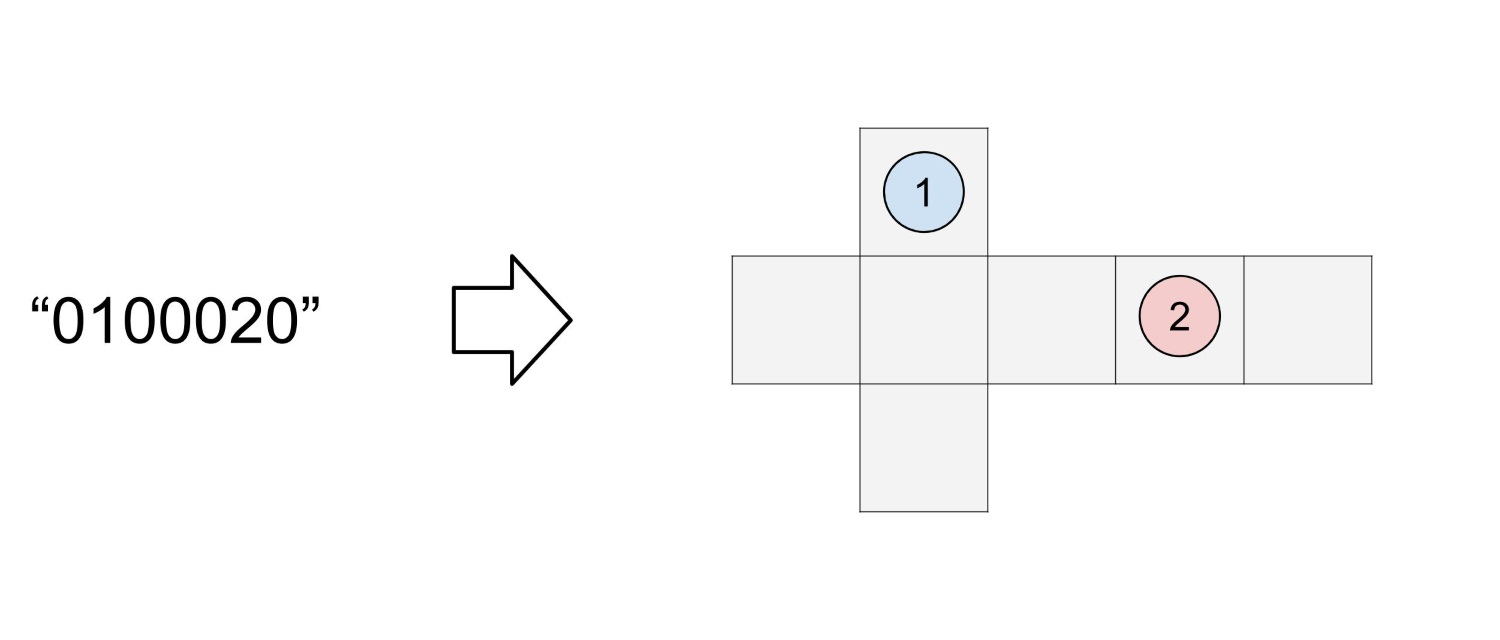
\includegraphics[height=4cm]{./Images/3_Playing_Field_Encoding.jpg}
        \caption{State string with equivalent playing field representation}
        \label{fig:field_mapping}
    \end{figure}


    The number of possible states is determined by the number of agents in the experiment and is equal to the number of unique permutations of agents and locations. It is calculated with the following formula:

    \begin{equation}
        N_{states} = \dfrac{m!}{(m-n)!}
    \end{equation}

    For an experiment with 1, 2 or 3 agents there are 7, 42 and 210 possible states, respectively. Given the somewhat low number of possible states, this study opted to implement the transition matrix as a direct state to state mapping, resulting in a square NxN matrix, N being the number of possible states. This trades a higher memory footprint for ease of implementation and interpretation. This particular implementation has a memory footprint proportional to N$^2$, in problems with a larger state space, one might opt to implement the transition table based on possible actions (Up, Right, Down, Left, and Stay) given that the matrix would increase to the order of N. Another, even more memory efficient implementation would be to store only the possible transitions in a list or dictionary. Given the sparse nature of the transition matrix, this option would greatly diminish the amount of memory necessary for running the learning process, at the expense of increased implementation complexity.

    Considering each agents only moves itself, the state transitions will be different for each agent. In this particular implementation it was decided to keep a separate transition table for each agent. These tables are calculated at the beginning of the experiment. For each agent, the program iterates over all the possible states and checks which moves are possible for said agent.

    The reward function grants agents 100 points for any action that transition them to the desired state, this includes the non-movement action of staying in the same place. Contrarily, agents are awarded negative 100 points for transitions that take them away from the desired state.

\section{Learning Policy} \label{sec:learning_policy}
    The learning policy selected for this study is the $\epsilon$-greedy policy. This policy relies on a dynamic value $\epsilon$, such that $0<\epsilon<1$, to determine an agent's strategy in a given state/time. The agent is to explore (i.e. take a random action) with $\epsilon$ probability, and exploit (i.e. take the action which has the highest expected return as per the Q-matrix) with (1-$\epsilon$) probability. The learning process starts with a predetermined $\epsilon$ value, which is gradually decreased after each learning episode. This means that when there is more uncertainty (i.e. at the beginning of the learning process, when not much is known regarding the environment), the agent is more prone to take random actions, exploring the possible state space and gathering feedback and "understanding" of the surrounding environment. Gradually, the more the agent knows regarding the environment, less often it takes random actions. This effectively has the result of directing the random exploration to regions surrounding the currently learned action policy. The selection of initial value and decay function for $\epsilon$ plays an important role in the performance of the learning process. If the decay is too slow, or the initial value is too high, the agent will keep exploring for longer possibly over exploring the problem space before converging to a policy, leading to longer training times. Conversely, if the decay is too fast (or the initial value is too low), the agent will converge to a policy faster, but this policy may be suboptimal as the problem space was underexplored. Naturally the optimal decay rate is dependent on the particular task being learned and the size of the state space. Striking this optimal balance is, therefore, an important step in the tuning process.

\section{Graphical Representation \& R Matrix} \label{sec:r_matrix}

    \begin{figure}[ht]
        \centering
        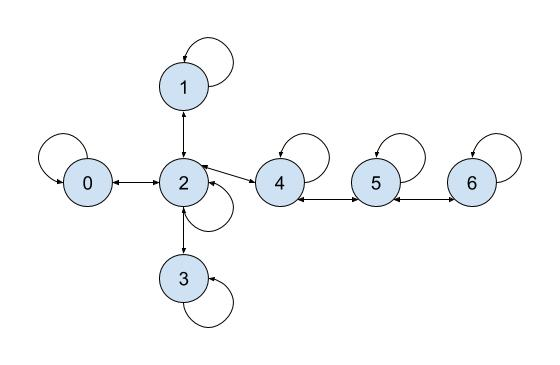
\includegraphics[height=4cm]{./Images/4_TransitionGraph.jpg}
        \caption{Base Transition Graph}
        \label{fig:transition_graph}
    \end{figure}

    The agents share the playing field and have the same movement rules, they also share a base movement graph. Figure \ref{fig:transition_graph} represent the shared transition graph between board locations. It is important to stress that, depending on the current board disposition, some transitions may not be available for a given agent. For example, an agent on location 6 may have it's 6$\rightarrow$5 transition blocked if there is another agent occupying location 5.

    As stated in section \ref{sec:transition}, the program makes use of this base transition graph to generate the full transition matrix. Since the study aims to analyze the behaviour of a multi-agent scenario, the agent's are deemed independent in terms of movement and policy. Hence, it was decided during implementation to have a separate transition matrix for each agent. Similarly, each agent has a separate R matrix associated with it. Even if, for the purposes of this study the agents are cooperative and share the same terminal state, their transitions into such final state are different given that their movement is ruled by the same constraints, but is not identical in terms of origin and destination states. The R matrixes are generated by the following steps:
    \begin{enumerate}
        \item Generate the transition matrix for that particular agent
        \item Set all transitions to have return of 0
        \item Set all transitions \textbf{away} from the desired terminal state to have reward of -100
        \item Set all transitions \textbf{into} the terminal state to 100
    \end{enumerate}

    Figure \ref{fig:r_matrix} shows the R matrix generated for agent \#1 in a experiment with a single agent.

    \begin{figure}[h]
        \centering
        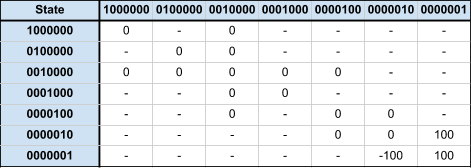
\includegraphics[height=4cm]{./Images/5_R_Matrix.png}
        \caption{R Matrix generated for experiment with a single agent}
        \label{fig:r_matrix}
    \end{figure}

\section{Q-Learning Parameters}\label{sec:params}
    The Q-Learning algorithm provides a some hyperparameters that may be tuned according to the task at hand and the limitations and opportunities associated with it. The two most prominent would be $\gamma$ and $\alpha$. This study presents additional parameters directly or indirectly related to Q-Learning (e.g. number of episodes, max steps per episode, $\epsilon$ decay rules), as well as parameters associated with the task itself (e.g. Number of agents, reward for reaching terminal state).

    \subsection{Discount Factor - $\gamma$}
        The discount factor ($\gamma$) main function is to weigh the probability of receiving expected future rewards. It is used as a multiplier to the maximum expected return of the next step, when updating the Q-Matrix. In a sense, it represents the certainty associated with eventually receiving future rewards. It's value may range from 0 to 1: 0 being no certainty at all, thus ignoring any expected return beyond the immediate step being taken. And 1 representing absolute certainty that future returns will match the expectation. For the initial experiment, $\gamma$ was set to \texttt{0.5}.

    \subsection{Learning Rate - $\alpha$}
        The learning rate parameter is used to control the rate at which the Q-Matrix is updated after a learning observation. As an analogy, it could be associated to the Q-Matrix's inertia. As with $\gamma$, $\alpha$'s values are between 0 and 1. As per the analogy, 0 would represent a scenario in which the Q-Matrix has infinite inertia, thus the Q-Matrix values remain the same, regardless of the feedback received from the observation. Oppositely, an $\alpha$ of 1 would represent a Q-Matrix with no inertia at all with it's values being completely replaced by the observations gathered at every step. For the initial experiment, $\alpha$ was set to \texttt{0.5}

    \subsection{Epsilon - $\epsilon$}
        The $\epsilon$ parameter refers to the $\epsilon$-greedy algorithm, which is used to select the actions taken by agents in the learning process. The results of such actions are then fed to the Q-Learning algorithm in the Q-Matrix update cycle. As stated in section \ref{sec:learning_policy} this experiment opted to rely on a commonly used pattern of multi-band $\epsilon$ decay. For the initial experiment the following values were used:
        \begin{itemize}
            \item Initial $\epsilon$: \texttt{0.999}
            \item Decay threshold (\texttt{r}): \texttt{0.5}
            \item Decay Rate 1 ($\epsilon$ $\geqslant$ \texttt{r}): \texttt{0.9995}
            \item Decay Rate 2 ($\epsilon$ $<$ \texttt{r} ): \texttt{0.995}
        \end{itemize}

    \subsection{Experiment duration - (\texttt{num\_episodes} and \texttt{max\_steps})}\label{sec:params:duration}
        \sloppy This study defines two stopping criteria regarding the learning experiments: \texttt{num\_episodes} and \texttt{max\_steps}. The former determines how many learning episodes are ran in total before analyzing the results. While the latter establishes a maximum amount of steps taken in a single learning episode before declaring the agents as "stuck" and terminating the episode. If the terminal state is reached before \texttt{max\_steps} are taken, the episode is also terminated. One detail that is important to stress is that, in this experiment, in a multi-agent scenario the terminal state is only considered as reached when every single agent has performed an action that results in reaching that state, thus collecting its reward. For the initial experiment, the following values were used: \texttt{num\_episodes}=5000 and \texttt{max\_steps}=30.

    \subsection{Reward/Penalty}
        In this study, the reward and penalty values are defined arbitrarily, given the abstract nature of the experiment. As noted in section \ref{sec:r_matrix}, the initial values for reward and penalty are 100 and -100, respectively.

    \subsection{Number of Agents - (\texttt{num\_agents})}
        For implementation purposes, the number of agents in a experiment is also configurable. The initial experiments take place with both 1 and 2 agents settings.

\section{Q-Matrix Update Cycle}
    Central to the Q-Learning algorithm is the Q-Matrix update cycle. After each step taken by an agent, it's associated Q-Matrix is updated. The new value for the origin($s$)/action($a$) pair ($Q(s,a)_{new}$) is calculated based on the old origin/action value ($Q(s,a)_{old}$); the reward/penalty observed ($r$); the maximum expected return (as per the current Q-matrix) for future actions($a'$) taken from the destination state ($s'$) $\Rightarrow$ $max_{a'} Q(s',a')$; and the learning parameters discount factor ($\gamma$) and learning rate ($\alpha$). The equation used for updating the value is:

    \begin{equation}
        Q(s,a)_{new} = Q(s,a)_{old} + \alpha*[r+\gamma*max_{a'} Q(s',a') - Q(s,a)_{old}]
    \end{equation}

    Implementation-wise the code, in Python, used for updating the Q-Matrix is the following:

\onecolumn
% Keep identation to left since \begin{python} respects current identation
    \begin{python}
def update_q_matrix(current_state, next_state, current_agent_id, earned_reward):
    # Get alpha and gamma from experiment settings
    alpha = EXPERIMENT['alpha']
    gamma = EXPERIMENT['gamma']

    # Get current agent's Q-matrix
    current_q = Q[current_agent_id]

    # Q(s,a)old
    old_expected_return = current_q.loc[current_state, next_state]

    # max a' Q(s',a')
    possible_next_moves = get_available_moves(next_state, current_agent_id)
    best_expected_return = max(current_q.loc[next_state, possible_next_moves])

    # Q(s,a)new
    new_expected_return = old_expected_return + alpha * (earned_reward + gamma * best_expected_return - old_expected_return)

    # Update value in current agent's Q-matrix
    current_q.loc[current_state, next_state] = new_expected_return
    \end{python}

\section{Initial Results}
    \subsection{Single agent}
        Initial results indicate that, for the 1 agent variant, the system is able to learn how to reach the terminal state. Figures \ref{fig:exp1:win_percent}, \ref{fig:exp1:steps} and \ref{fig:exp1:updates} show, over the course of the experiment, respectively: the win \% (i.e. episode did reach terminal state); number of steps per episode; and number of updates to Q matrix per step taken. All graphs were calculated with a moving window of 100 episodes to smooth out variations due to randomized initial condition and noise in case of boolean values (e.g. win \%). The graphs also contain the epsilon value per episode, which was not smoothed out with a moving window. Figure \ref{fig:exp1:win_percent} indicates that after a little more than 1000 episodes, the agent is able to consistently reach the terminal state every single time, while \ref{fig:exp1:steps} indicate that not only the agent consistently reaches the terminal state, but does so with increasing efficiency, reaching an average of 4 steps per episode. Finally figure \ref{fig:exp1:updates} indicates strong activity in updating the Q-Matrix in the beginning of the experiment. Given that the decrease in update activity coincides with the dramatically increase in exploitation probability it is not possible to determine whether the root cause of such phenomenon is due to complete convergence of the Q-Matrix, or due to a specific path being preferred and continuously exploited. Given the simplicity of the maze for a single agent it is arguable that both phenomena occur in tandem since, for each initial state, there is a single direct path towards the terminal state.
        \begin{figure}[h]
            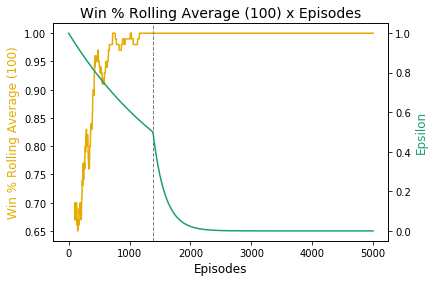
\includegraphics[height=4cm]{Images/exp_1/1_win_percent.png}
            \caption{Percentage of episodes able to reach terminal state in single agent experiment}
            \label{fig:exp1:win_percent}
        \end{figure}
        \begin{figure}[h]
            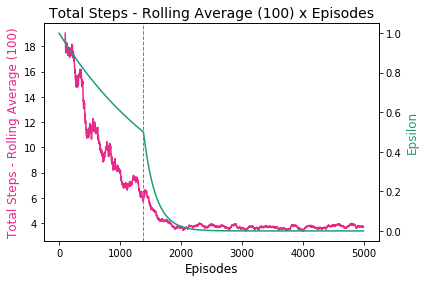
\includegraphics[height=4cm]{Images/exp_1/2_total_steps.png}
            \caption{Steps taken per episode in single agent experiment}
            \label{fig:exp1:steps}
        \end{figure}
        \begin{figure}[h]
            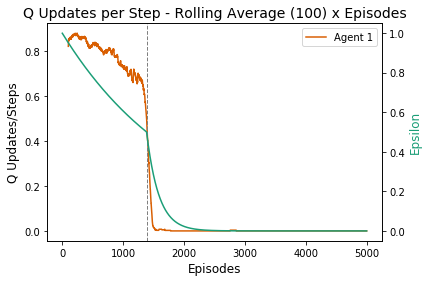
\includegraphics[height=4cm]{Images/exp_1/3_updates_per_step.png}
            \caption{Number of updates to Q Matrix per step taken in single agent experiment}
            \label{fig:exp1:updates}
        \end{figure}

    \subsection{Two agents}
        The initial results for experiments with two independent agents show that they fail to learn the correct path to terminal state. Figures \ref{fig:exp2:win_percent} and \ref{fig:exp2:steps} indicate how the agents are not able to reach the terminal state on a consistent basis, even after epsilon is near 0, meaning the agents are expected to always chose the action with the highest expected reward (i.e. the one that leads them faster to the terminal state). While figure \ref{fig:exp2:updates}, indicates that  there is little activity in agent 1's Q-Matrix, which appears to converge well before the shift to exploitation and also sooner than the experiment with a single agent. The figure also indicates continuous (an erratic) activity in agent 2's Q-Matrix, well after the shift to exploitation.
        \begin{figure}[h]
            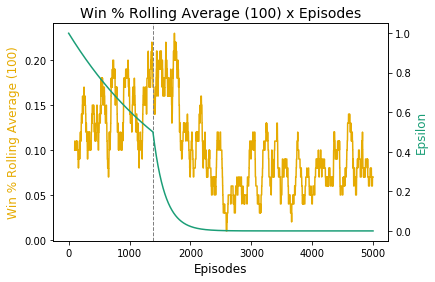
\includegraphics[height=4cm]{Images/exp_2/1_win_percent.png}
            \caption{Percentage of episodes able to reach terminal state in two-agent experiment}
            \label{fig:exp2:win_percent}
        \end{figure}
        \begin{figure}[h]
            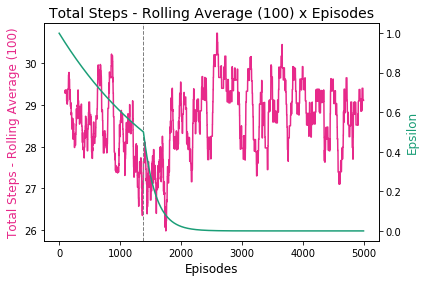
\includegraphics[height=4cm]{Images/exp_2/2_total_steps.png}
            \caption{Steps taken per episode in two-agent experiment}
            \label{fig:exp2:steps}
        \end{figure}
        \begin{figure}[h]
            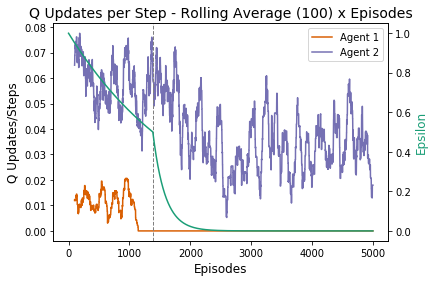
\includegraphics[height=4cm]{Images/exp_2/3_updates_per_step.png}
            \caption{Number of updates to Q Matrix per step taken in two-agent experiment}
            \label{fig:exp2:updates}
        \end{figure}

\section{Further Tests}\label{sec:further_tests}
    In order to visualize the influence each parameter has on the learning process, further experiments were ran by varying each parameter individually. Unless otherwise specified, the remaining parameters were kept at the values indicated in section \ref{sec:params}

    \subsection{Experiment duration}
        As specified in section \ref{sec:params:duration}, the experiment duration dictates how many episodes are ran per experiment. Considering that the scenario is deterministic, static, and the state-space is finite and small (i.e.: feasibly exhaustible), the experiments are expected to converge after a certain number of learning episodes and remain stable after that. Following that logic, in order to study the behaviour of agent's learning, it suffices to constrain the number of episodes to be enough to show the learning stage and a sample of the post converged regime. In order to speed up the simulations while still being able to represent the whole phenomenon, the number of episodes used is lowered to 2500. In some specific cases this number may not be enough to show the complete picture, such instances are dealt on an ad-hoc basis by increasing the number of episodes, as needed, for that particular experiment.

    \subsection{$\alpha$ values}
        Experiments were ran with six different values for $\alpha$, ranging from 0 to 1 (included). The results can be seen in figures \ref{fig:exp3:win_percent} and \ref{fig:exp3:win_percent_two}
        \begin{figure}[h]
            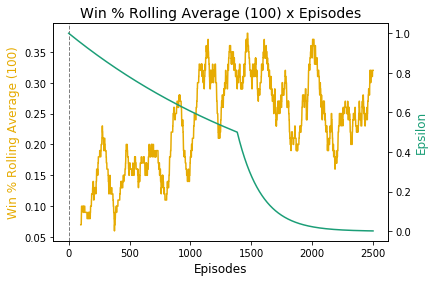
\includegraphics[height=4cm]{Images/exp_3/1_win_percent.png}
            \caption{Win \% progression with varying $\alpha$ - Single agent}
            \label{fig:exp3:win_percent}
        \end{figure}

        \begin{figure}[h]
            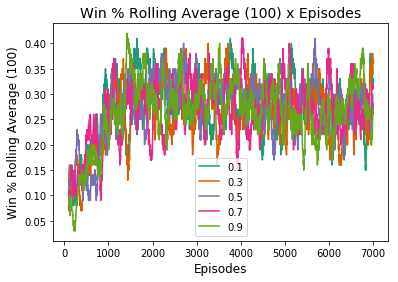
\includegraphics[height=4cm]{Images/exp_3/2_win_percent.png}
            \caption{Win \% progression with varying $\alpha$ - Two agents}
            \label{fig:exp3:win_percent_two}
        \end{figure}


    \subsection{$\gamma$ values}
        Experiments were ran with six different values for $\gamma$, ranging from 0 to 1 (included). The results can be seen in figures \ref{fig:exp4:win_percent} and \ref{fig:exp4:win_percent_two}
        \begin{figure}[h]
            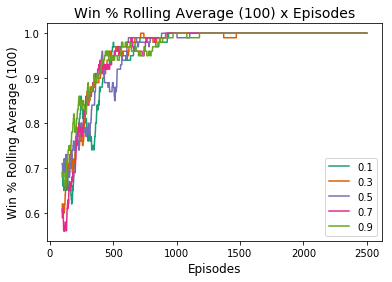
\includegraphics[height=4cm]{Images/exp_4/1_win_percent.png}
            \caption{Win \% progression with varying $\gamma$ - Single agent}
            \label{fig:exp4:win_percent}
        \end{figure}

        \begin{figure}[h]
            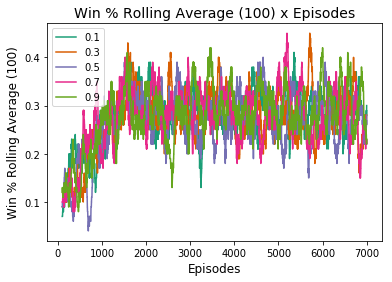
\includegraphics[height=4cm]{Images/exp_4/2_win_percent.png}
            \caption{Win \% progression with varying $\gamma$ - Two agents}
            \label{fig:exp4:win_percent_two}
        \end{figure}

    \subsection{Maximum Episode duration - \texttt{max\_steps}}
        Experiments were ran with the following \texttt{max\_steps} values: [4, 6, 8, 10, 30, 60, 100]. The lower bound of 4 was selected as it represents the maximum number of steps needed for a single agent to reach terminal state if following the optimal policy. The upper bound of 100 represent a value two orders of magnitude larger. The results are shown in figures \ref{fig:exp5:win_percent} and \ref{fig:exp5:win_percent_two}

        \begin{figure}[h]
            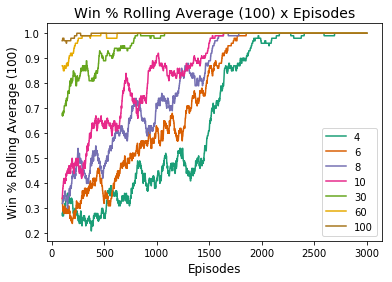
\includegraphics[height=4cm]{Images/exp_5/1_win_percent.png}
            \caption{Win \% progression with varying \texttt{max\_steps} - Single agent}
            \label{fig:exp5:win_percent}
        \end{figure}

        \begin{figure}[h]
            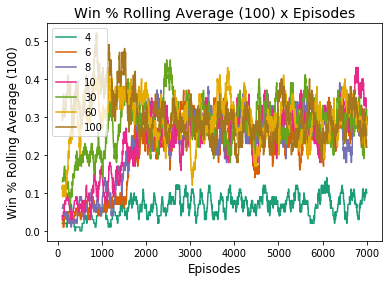
\includegraphics[height=4cm]{Images/exp_5/2_win_percent.png}
            \caption{Win \% progression with varying \texttt{max\_steps} - Two agents}
            \label{fig:exp5:win_percent_two}
        \end{figure}

    \subsection{$\epsilon$ decay}
        Regarding the $\epsilon$ decay, 2 different tests were done: a) Vary the threshold at which the decay changes; and b) Vary the $\epsilon$-decay rates.

        \begin{figure}[h]
            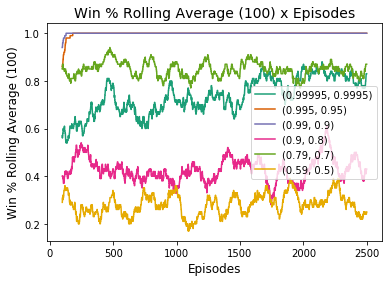
\includegraphics[height=4cm]{Images/exp_6/1_change.png}
            \caption{Win \% progression with varying $\epsilon$ decay change threshold  - Single agent}
            \label{fig:exp6:change}
        \end{figure}

        \begin{figure}[h]
            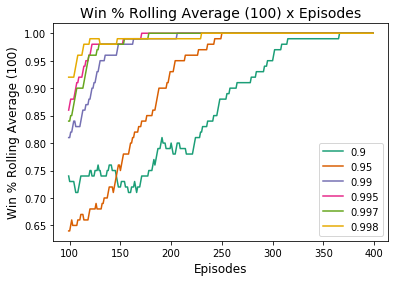
\includegraphics[height=4cm]{Images/exp_6/2_threshold.png}
            \caption{Win \% progression with varying $\epsilon$ decay rate - Single agent}
            \label{fig:exp5:threshold}
        \end{figure}


\section{Quantitative Analysis}\label{sec:quant_analysis}
    From the experiments results shown in section \ref{sec:further_tests}, the first conclusion that can be drawn is that, regardless of the changes in hyperparameters presented, the Q-Learning algorithm, as implemented, is unable to converge to a solution when dealing with 2 independent agents. The rolling win \% remains noisy and shows no sign of move towards an increase in the win ratio in all cases observed. Conversely, in the single agent scenario, the algorithm converges to optimal solution in all cases.

    Changing either $\gamma$ or $\alpha$ produced no change whatsoever in the convergence to the optimal solution, not even in the speed at which the agent converges. They did however produce changes in the duration of update activity in the Q table. Such duration was inversely proportional to $\alpha$, and directly proportional to $\gamma$.
    Regarding individual episodes' duration, increasing the maximum duration had the effect of proportionally increasing the win \%
    Finally, observing the effects of variations in the $\epsilon$ parameters, it can be said that, for this particular setting, lowering the both decay rates had the effect of reducing the amount of episode needed to reach 100\% win rate.

\section{Qualitative Analysis - Single Agent}
    Further examining the results discussed in section \ref{sec:quant_analysis} and crossing them with knowledge of how the Q-Learning algorithm works, it is possible to reach explanations as to why such behaviours manifest themselves.

    \subsection{Maximum Episode duration - \texttt{max\_steps}}
        Differently from the experiment duration, which only varies the observed window of the learning process, the maximum episode duration may affect the learning process to the extent that longer episodes increase the chance of randomly reaching the terminal state as well as increase the probability of propagating the return expectation throughout the Q-Matrix as more actions are taken per episode. So, if we are to measure the win \% in terms of episodes, the average win \% is expected to be directly correlated to the maximum number of steps allowed per episode.

    \subsection{$\alpha$ and $\gamma$}\label{sec:quali:gamma}
        Initially, it may seem strange that two of the most prominent hyperparameters in Q-Learning have little effect in the rate at with the algorithm converges in terms of win \%. This behaviour, however, can be fully explained by the inner workings of the Q-Learning algorithm coupled with the topology of the playing field. Such invariance to changes in $\alpha$ and $\gamma$ can be explained by four factors:
        \begin{enumerate}[a)]
            \item the field is a narrow corridor with no loops
            \item there is a single positive reward source/state and no punishment(negative reward) is ever given
            \item the learning starts with a Q-Table with all actions expecting 0 reward
            \item the setting is completely deterministic
            \item Q-Matrix is updated after each action
        \end{enumerate}
        The playing field topology is such that, for any 2 locations, there is only a single path that joins them without backtracking. In essence, this means that, for each given location, there is only a single path to be learned to reach the terminal state. Being the playing field deterministic, and the Q-Matrix updated after each step means that the values in the Q-Matrix will monotonically increase until reaching their post convergence values. Based on this, the expected reward is propagated backwards from the terminal state to each location through multiple learning episodes in a way that actions leading to states closer to the terminal are guaranteed to always have higher rewards than ones leading away at any given moment in the learning process. Changes in $\alpha$ and $\gamma$ have the effect of changing the absolute values for actions within the Q-Matrix, but not their relative values towards other actions and, consequently, the decisions taken by a greedy agent.

    \subsection{Decay Rate - $\epsilon$}
        This scenario favors lower decay rates, this makes sense given the simplicity of the task to be learned.
        The $\epsilon$-greedy policy has the effect of slowly increasing the greediness of the agent so that the randomness is constrained to state/action pairs neighbouring the slowly learned optimal policy. This is necessary in situations with a state/action space large enough that exhausting it is not feasible with the available computing power.
        Given the behaviour described in section \ref{sec:quali:gamma}, it is known that it is not necessary to wait for the Q-Matrix to fully converge (i.e. reach an equilibrium), as a small change in the Q-Matrix is suffices to lead a greedy agent towards the terminal state. The size of the board, and therefore the state-action pair space, is such that it can be exhausted by brute force with a somewhat low processing power available. Thus, having the agent taking random actions is enough to fully explore the space and converge the Q-Matrix in considerably fast fashion. Given this, the benefits of using an $\epsilon$-greedy policy are greatly diminished. In this sense, the lower decay instances providing faster convergence to a 100\% win rate is merely a product of the agents' increased greediness, rather than the algorithm learning considerably faster.


\section{Qualitative Analysis - Two Agents}
    As observed in section \ref{sec:quant_analysis}, the implemented Q-Learning algorithm was unable to reach an optimal policy in a two agents scenario. This can be explained in terms of the topology of the playing field and movement rules applied. The game ends whenever both agents perform a move to the terminal state. Given the field topology this can only be reached with the following final moves:


    This collection of moves means that the only direct move Agent 1 can take to reach terminal state is staying in place once Agent 2 has moved into position. In other words, Agent 1 is not able to fully traverse the state space with only actions of her own - the state space is detached into 2 groups. Considering that the Q-Learning'sample backup is only a single step deep, there is no way for this action's reward to propagate backwards through the Q-Matrix from one group to the other. This can be evidentiated by inspecting Agent 1's Q-Matrix after convergence. It expects the correct reward for the winning move (i.e. Staying in place when in state "0000021"), but expects 0 reward for all other state/action pairs. In other to circumvent this limitation there possible alternatives would be: have the agent's share information; and implement a learning algorithm that is able to propagate rewards backwards through multiple steps rather than a single one (e.g.: TD-Learning, Monte Carlo).

\section{Advanced Reinforcement Learning Techniques}
    \subsection{TD($\lambda$)-learning}
    The aim of this study is to observe the effects of independent agents collaborating in a multi-agent scenario, thus instead of implementing information sharing techniques, I decided to implement a RL technique which propagates rewards further back than a single action. The technique chosen was TD($\lambda$) learning with eligibility traces. This technique updates the complete Q-Matrix every single step by leveraging a separate matrix used to track each state/action pair's eligibility based on how recent said pair was visited. A new hyperparameter $\lambda$ is introduced to control the speed of decay of the eligibility traces. The intuition behind this choice is that by being able to propagate rewards further back than a single step, the scenario with 2 independent agents will be able to converge to an optimal winning policy. The results for various values of $\lambda$ can be seen in figure \ref{fig:expII:winning}

    \begin{figure}[h]
        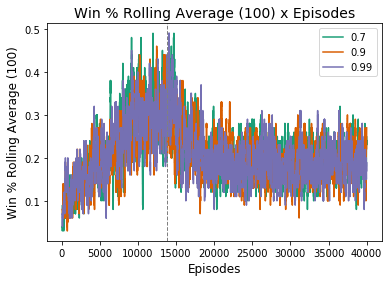
\includegraphics[height=4cm]{Images/exp_II/1_winning.png}
        \caption{Win \% progression vs $\lambda$ - Two agents}
        \label{fig:expII:winning}
    \end{figure}

    As the results clearly show, TD($\lambda$) by itself is not able to reach an optimal policy in the two agent scenario. MOst interestingly is how the win rate keeps changing considerably after the agents enter into greedy mode. Upon further consideration and studies, it was found that this phenomenon happens due to the turn-by-turn nature of the game. From the perspective of an outside observer, the environment is static because the state only changes due to an action by either agent. However, from the perspective of each single agent, it is a dynamic environment because the state at which they take the next step is different from the state reached by her previous step. In practical terms, in TD($\lambda$) this means that the Q-Matrix will be updated in disorderly fashion, for each agent an state/action pair is updated while taking into account possible future action from states that said agent might not be visit in this episode. The backpropagating nature of Q and TD($\lambda$) Learning means that, for scenarios with only positive rewards, when calculating an error the best expected return for a future action taken from state \texttt{s} is larger than the expected return from an action leading to state \texttt{s}. Thus the error is always positive and the expected returns for all state/action pairs monotonically increase until reaching convergence. By the dynamicity introduced by two agents taking turns, this will not hold true. A side effect of this can be observed in the win \% decreasing after the agents enter into greedy mode. What little was learned from the environment is gradually "unlearned" by the agent's observing 0 reward for their general actions and decreasing the values in the Q-Matrix.

    \subsection{Hyperstate Q-Learning}
    To circumvent the issued caused by the dynamic environment observed by the individual agents, a small but powerful change was introduced to the Q-Learning implementation. When calculating the individual error for a given state/action pair, instead of comparing it with the best expected return for actions taken from the next state, the algorithm compares the old expected return with the best expected return for actions taken from the next \textbf{hyperstate}. In this context an hyperstate is defined as the collection of states reachable by actions taken from the other agent in her turn. In practical terms the next hyperstate is the group of states an agent may find herself in when their next turn is due. This has the double effect of \textbf{i)} removing the observed dynamicity of the environment by taking into account all possibilities for the next turn and \textbf{ii)} eliminating the detached nature of the state space that was introduced in the multi-agent scenario.

    \begin{figure}[h]
        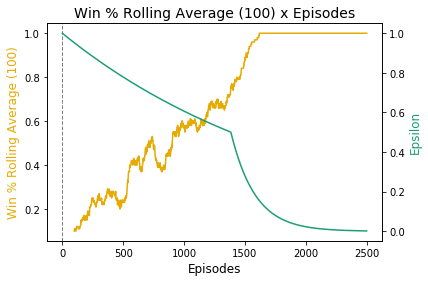
\includegraphics[height=4cm]{Images/exp_III/1_winning.png}
        \caption{Win \% progression - Hyperstate Q-Learning - Two agents}
        \label{fig:expIII:winning}
    \end{figure}

    The results of the hyperstate Q-Learning (figure \ref{}) clearly show that this technique lead to the optimal policy convergence. It is important to note 2 important points regarding this implementation:
    \begin{enumerate}[1)]
        \item It was based on standard Q-Learning, so the algorithm converges even when updating the Q-Matrix after each step (i.e. there is no need for holistic techniques such as TD($\lambda$))
        \item While this technique is able to treat the environment as static in the two agents scenario, the size of the next hyperstate increases exponentially with the number of players in the field. Thus for a large number of players this technique would become computationally too expensive and a different approach would be needed.
    \end{enumerate}

\section{Q-learning and Psychological Error Correction Models}

\section{Error Correction Implementation Proposal}

\end{document}